\documentclass[12pt]{article}
\usepackage[a4paper, margin=1in]{geometry}
\usepackage{graphicx}
\usepackage{amsmath}
\usepackage{hyperref}
\usepackage{titlesec}
\usepackage{setspace}
\usepackage{enumitem}
\usepackage{natbib}
\usepackage{tikz}
\usepackage{amssymb}
\usepackage{float}
\usepackage{booktabs}
\usepackage{todonotes}
\usetikzlibrary{trees}
\titleformat{\section}{\normalfont\Large\bfseries}{\thesection.}{1em}{}
\titleformat{\subsection}{\normalfont\large\bfseries}{\thesubsection.}{1em}{}

\title{Network Games and Agricultural Collectivization in China}
\author{Xinkai Xu, Liming Lin, Zihao Liu}
\date{\today}

\begin{document}

\maketitle
\onehalfspacing

\begin{abstract}
This project uses the framework of network games to analyze incentive structures and behavioral dynamics in the context of Chinese agricultural collectivization during the 1960s and 1970s. Starting from a baseline model of small reciprocal production teams, we incrementally build up to more complex systems. Firstly, we expand the network by conecting different teams, allowing for inter-team interactions. Then we add signaling games to capture the information assymetries and communications among agents. Finally, we introduce external shocks to the system, such as natural disaster, to study the reactions of different network structures. And we find that ...
\end{abstract}

\section{Introduction}
The process of agricultural collectivization in China has long been analyzed through the lens of free-rider problems, where the expansion from small mutual-aid groups to large communes led to decreased efficiency due to weakened individual incentives. In this paper, we offer a complementary explanation grounded in network theory and behavioral interactions: we argue that peer effects—the informal social pressures and mutual influences among connected individuals—diminish in larger collectives, leading to reduced effort and lower overall productivity.

In smaller groups, individuals are closely connected, better informed about one another’s behaviors, and more likely to internalize social expectations. This fosters a strong peer monitoring effect, where effort decisions are mutually reinforced. However, as collectives grow, these connections become sparser and information about peers becomes incomplete. The weakening of relational ties reduces the salience of social norms, thereby diluting the peer effect that sustains cooperation.

Building on this framework, we introduce a signaling model to capture the government’s strategic role in influencing behavior under incomplete information. Through public signals—such as praising model workers (high-type signal, h) or criticizing slackers (low-type signal, l)—the state can shape agents' beliefs about their peers’ effort levels. These signals serve as proxies for missing information and potentially restore peer effects by coordinating expectations and encouraging conditional cooperation.

Our analysis combines network game theory with a behavioral signaling mechanism to explore the interaction between group size, informational frictions, and state propaganda. We show how the erosion of peer effects in large networks can be partially mitigated through targeted signaling, and we highlight the institutional implications for collective governance and social enforcement.\\

\section{Base Model: The Small Network within a Commune}
In the early stages of rural collectivization, agricultural production was organized through mutual-aid teams, typically consisting of a handful of neighboring households. These small groups were built upon existing social ties, such as kinship, proximity, and shared village identity. Within such closely-knit settings, individuals were able to observe each other’s behavior directly, fostering a high degree of mutual monitoring and reciprocal expectations. This justifies the modeling assumption of complete information, where each agent has accurate knowledge of their peers’ effort levels. In this environment, peer effects are strong, and cooperative behavior is sustained by informal social norms and reputational incentives.\\

Let $I = \{1, 2, \dots, n\}$ denote the set of players, $n > 1$, connected by a network $G$. We use matrix $G$ to track the connections in this network. We define $g_{ij} = 1=g_{ji}$ if $i$ and $j$ are linked to each other, and $g_{ij} = 0$ otherwise.  We also set $g_{ii} = 0$. The neighborhood of the individual $i$ is the set given by $[ N_i := j \mid g_{ij}] = 1$. Therefore, $|N_i|$, the cardinality, which is $\sum_j g_{ij}$, is called the \textbf{degree} of $i$.\\

We use the following quadratic utility function to capture the \emph{strategy complementarity}:
\[
U_i(x_i, x_{-i}, G_i) = \alpha x_i - \frac{1}{2} x_i^2 + \beta x_i \sum_j g_{ij}x_i  x_j,
\]

where $\alpha$ is the marginal return to effort $x_i$, and $\beta$ is the strength of strategic interactions.

We assume $\beta > 0$, so that we have
\[
\frac{\partial^2 U_i(x_i, x_{-i}, G_i)}{\partial x_i \partial x_j} = \beta g_{ij} > 0,
\]
which reflects strategic complementarity in efforts.

In small groups with $n$ players in a network, people know each other well, and it is reasonable to assume network $G$ is a \textbf{complete network} and players have full information.

\begin{figure}[H]
  \centering
  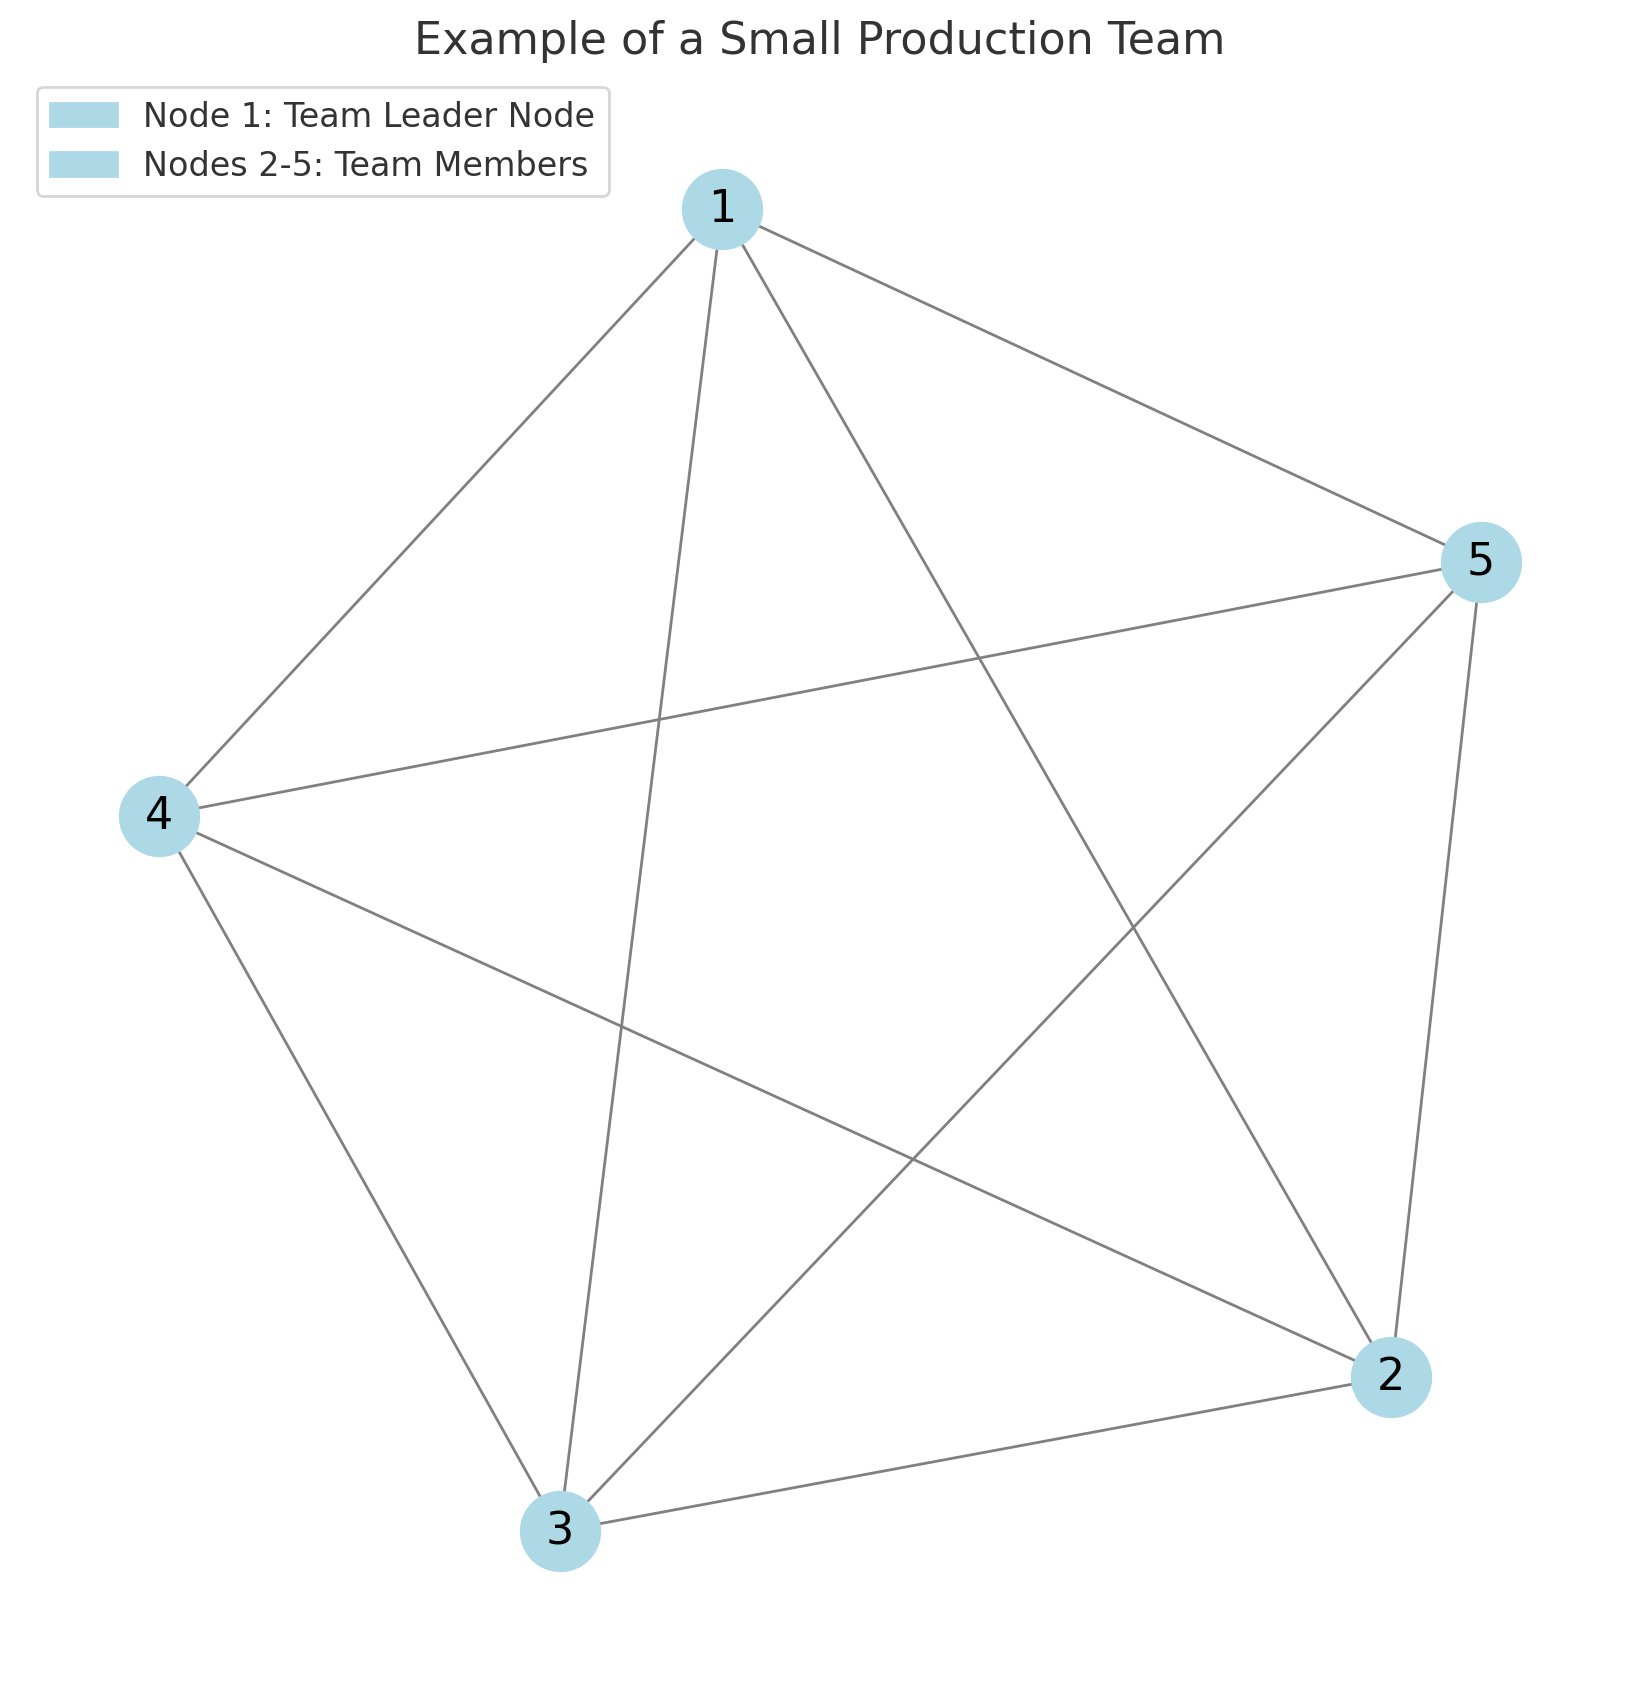
\includegraphics[height=0.6\textwidth]{small network1.png}
  \caption{Example of a Small Production Team}
  \label{fig:small-team}
\end{figure}

In equilibrium, each agent maximizes their utility. By the FOC, we get:
\[
x_i^* = \alpha + \beta \sum_j g_{ij}x_i x_j. \tag{2}
\]

Since $G$ is a complete network, everyone has the same degree. We assume total effort is  
\[
\bar{x} = \sum_i x_i,
\]
and so:
\[
x_i^* = \alpha + \beta \left( \sum_{j \neq i} x_j^* \right) = \alpha + \beta(n - 1)\bar{x}. \tag{3}
\]

Assuming symmetry, i.e., $x_i^* = \bar{x}$ for all $i$, we get:
\[
x_i^* = \frac{\alpha}{1 - \beta(n - 1)}.
\]

Then, in a small group, the utility of agent $i$' is given by:
\[
\frac{\alpha^2}{\beta + 1 - n\beta} - \frac{1}{2} \left( \frac{\alpha}{(\beta + 1 - n\beta)} \right)^2 + \beta(n - 1) \left( \frac{\alpha}{\beta + 1 - n\beta} \right)^2. \tag{4}
\]


\section{Large Networks}
\subsection{Large Network with Without Signaling}
Now we move to the large network setting where there are multiple small groups. And in each small complete network, there is one node that represents the leader of the small group. Between the small groups, there are indirect connections among the small group leaders through a central node the represents higher level government.\\
By this construction, we have three types of players with different degrees.  
We assume $N = nk + 1$, where $n$ is the number of players in a small group, $k$ is the number of small groups.

\begin{itemize}
    \item Type 1: $(n-1)$ degrees (internal to small group)
    \item Type 2: $k$ degrees (one connection to each small group leader)
    \item Type 3: $n$ degrees (small group leader)
\end{itemize}

\begin{figure}[H]
  \centering
  \includegraphics[width=0.7\textwidth]{large network1.png}
  \caption{Example of a Large Network}
  \label{fig:large-network}
\end{figure}
Incomplete information about $\beta$ without signals.

We assume $\beta$ takes two possible values: $\beta = \{\beta_l,\beta_h\}$ where $\beta_l < \beta_h$. 

We assume each agent holds a belief for $\beta$.

They share a common prior:

\[
\mathbb{P}(\beta = \beta_l) = p, \quad \mathbb{P}(\beta = \beta_h) = 1-p
\]

Therefore we assume there is no communication between players, and the network does not affect the value of $p$.

Then:

\[
\mathbb{E}[x_i] = \alpha - \sum_{j} g_{ij} \mathbb{E}[x_j] + \mathbb{E}[\beta] p_i
\]

where:

\[
\mathbb{E}[\beta] = p \beta_l + (1-p) \beta_h
\]

Also:

\[
\mathbb{E}[x_i] = x_i
\]

Thus:

\[
\alpha - x_i + \mathbb{E}[\beta] p_i - \sum_{j} g_{ij} x_j = 0
\]

\vspace{1em}

Thus:

\[
x_i^* = \alpha + \mathbb{E}[\beta] + \sum_{j=1}^{n} g_{ij} x_j
\]

where $G$ is the network matrix.

\vspace{1em}

The solution is given by:

\[
x^* = \alpha (I_n - \mathbb{E}[\beta] G)^{-1} \mathbf{1}
\]

where $I_n$ is the $n \times n$ identity matrix.

$G$ is the same network matrix as before.

\vspace{1em}

We assume that:

\[
\mathbb{E}[\beta] \leq \frac{1}{\lambda_{\text{max}}(G)}
\]

where $\lambda_{\text{max}}(G)$ is the largest eigenvalue of the network $G$.

\vspace{1em}

Moreover:

\[
(I_n - \mathbb{E}[\beta] p G)^{-1} = P_G \left( I - \mathbb{E}[\beta] p D_G \right)^{-1} P_G^{-1}
\]

where:

\[
G = P_G D_G P_G^{-1}
\]

and $D_G$ is the diagonal matrix of eigenvalues of $G$:

\[
D_G = 
\begin{pmatrix}
\lambda_1 & 0 & \cdots & 0 \\
0 & \lambda_2 & \cdots & 0 \\
\vdots & \vdots & \ddots & \vdots \\
0 & 0 & \cdots & \lambda_n
\end{pmatrix}
\]
Given the structure of the network, here is the $G$ matrix that represents the connections between players:
\begin{figure}[H]
  \centering
  \includegraphics[width=0.7\textwidth]{Default_Large_Network_Labeled.png}
  \caption{Adjacency matrix $G$ for the default 16-player network}
  \label{fig:G-matrix}
\end{figure}
So the 1st, 9th, and 12th rows are the leaders of the small groups, while the 16th row (the last row) is the central node that connects all the small group leaders. The rest are the members in the small groups.\\
Then we calculate the eigenvalues of the $G$ matrix. (See in appendix) The largest eigenvalue is $\lambda_{\text{max}}(G)  \approx 4.1622$ and thus the upperbound for $E[\beta] = \frac{1}{\lambda_{max}(G)} \approx 0.24$.\\
\subsubsection*{The Effects of $E[\beta]$ on Equilibrium Efforts}
We want to see how the equilibrium effort $x^*$ changes with the value of $E[\beta]$. However, it is very diffucult to compute with the differentiation, so here we just plug in $E[\beta]=0.2,0.1$\\
\begin{table}[H]
  \centering
  \begin{tabular}{lcc}
  \toprule
  \textbf{Player Type} & \textbf{\( x^* \) when \( E[\beta] = 0.2 \)} & \textbf{\( x^* \) when \( E[\beta] = 0.045 \)} \\
  \midrule
  Small Group Leader       & 6.67 & 1.27 \\
  Small Group Member       & 5.83 & 1.22 \\
  Central Leader (Player 16) & 5.00 & 1.17 \\
  \bottomrule
  \end{tabular}
  \caption{Equilibrium actions \( x^* \) under different values of \( \beta \)}
  \label{tab:xstar-beta}
  \end{table}
The table above confirms that the equilibrium effort \( x^* \) is increasing in \( E[\beta] \). This is because the higher the value of \( E[\beta] \), the more likely the players are to believe that their neighbors are also putting in effort, which leads to a higher equilibrium effort. Besides, the results also show that group leaders have the highest equilibrium, following by group members and central leader, corresponding to the fact that the group leaders have the highest numbers of nodes connected, while the central leader has the least.\\
\subsubsection*{The Effects of $p$ on Equilibrium Efforts}
More importantly, we want to investigate how the equilibrium effort \( x^* \) changes with the value of \( p \) which is the probability of being a high type player. Here we return to the original equation for $E[\beta]$ which equals $p\beta_h+(1-p)\beta_l$. We assume $\beta_l=0.03$ and $\beta_h=0.06$. (So the $p=0.5$ case will have the same $E[\beta]$ as above.)  Again, doing differentiation is complicated so we plug in several possible values for $p \in [0,1]$\\
\begin{table}[H]
  \centering
  \begin{tabular}{lccc}
  \toprule
  \textbf{Player Type} & \textbf{\( x^* \) at \( p = 0.1 \)} & \textbf{\( x^* \) at \( p = 0.5 \)} & \textbf{\( x^* \) at \( p = 0.9 \)} \\
  \midrule
  Small Group Leader        & 1.19 & 1.27 & 1.37 \\
  Small Group Member        & 1.15 & 1.22 & 1.30 \\
  Central Government (Player 16) & 1.12 & 1.17 & 1.23 \\
  \bottomrule
  \end{tabular}
  \caption{Equilibrium actions \( x^* \) as a function of \( p = \mathbb{P}(\beta = \beta_h) \)}
  \label{tab:xstar-vs-p}
  \end{table}
The table above shows that the equilibrium effort \( x^* \) is increasing in \( p \) which is aligned with the strategic complementarity.\\  
\subsection{Large Network with Signaling}
We move to a large network setting where each household only knows its own number of neighbors (degree) and forms beliefs over others' behavior. The model assumes strategic complements or substitutes depending on the distribution mechanism and social context.

There are $M \gg n$ players now. In this case, we treat $\beta$ as important information to capture the feature that in large groups, an agent does not know their neighbors' neighborhoods well.  
This uncertainty introduces people's incomplete information about $\beta$.

We assume that $\beta$ can only take two values, $\beta_L$ or $\beta_H$.  
All individuals share a common prior:
\[
\Pr(\beta = \beta_H) = p, \quad p \in (0,1)
\]

Individuals receive two signals which are not always correct.  
We define:
\[
\Pr(s_i = 1 \mid \beta = \beta_H) = q_1, \quad \Pr(s_i = 1 \mid \beta = \beta_L) = q_2
\]
where $s_i = 1$ and $s_i = -1$ denote the event that agent $i$ has received signal $1$ and $-1$, respectively.

Besides, we assume that the network is no longer a complete network.  
It is given by a graph


The idea is that a large network is composed of several small complete networks.  
And in each small complete network, there is one person who connects with leaders of the large group.

There are three types of players with different degrees.  
We assume $N = nk + 1$, where $n$ is the number of players in a small group, $k$ is the number of small groups.

\begin{itemize}
    \item Type 1: $(n-1)$ degrees (internal to small group)
    \item Type 2: $k$ degrees (one connection to each small group leader)
    \item Type 3: $n$ degrees (small group leader)
\end{itemize}

The utility function is the same for three types of players, given by:

\[
u_i(x_i, x_{-i}) = \alpha_i x_i - \frac{1}{2}x_i^2 + x_i\left( \sum_j g_{ij} x_j \right)
\]

By the first order condition, we get:
\[
x_i^* = \alpha + \beta \sum_{j = 1} g_{ij} x_j^*
\]

We define:
\[
b(\beta, G) = \sum_{k=0}^{\infty} \beta^k G^k I_n = (I_n - \beta G)^{-1} l_n,
\]
where \( I_n \) is the identity matrix \( n \times n \) and \( l_n \) is the vector \( n \times 1 \) of 1.

When agent $i$ receives signal $s_i = l$, his utility function satisfies:


\[
\mathbb{E}[x_i \mid s_i = l] = \alpha \, \mathbb{E}[x_i \mid s_i = l]
-\frac{1}{2}\mathbb{E}[x_i^2|[s_i=l]]+ \sum_{j = 1}^n g_{ij} x_i\, \mathbb{E}[x_j \mid s_j = t]
\]
\[
= \alpha \, x_i(l) - \frac{1}{2} x_i(l)^2 + \sum_{j=1}^{n} g_{ij} \, x_i(l) \, \mathbb{E}\left[ \beta \, x_j \mid s_j = l \right]
\]


Thus:
\[
x_i = \alpha_i(l) + \sum_j g_{ij} \mathbb{E}[x_j \mid s_i = l]
\]

By the first order condition on $x_i(l)$, we get:
\[
\alpha -x_i^*(l) +\sum_{j=1}^{n} g_{ij} \mathbb{E}[\beta x_j^* \mid s_i = l]=0
\]

When agent $i$ receives signal $s_i =l$, for each possible $j$ we have:
\[
\mathbb{E}(\beta_j x_j \mid s_i = l) = \sum_{t=1}^{2} \\
\sum_{m=1}^{2} \beta_{mx_j}(t) P\{\beta = \beta_m \cap s_j = l\}
\]
\[
= \beta_{\max} \sum_{t=1}^{2} \left( P\left( \{\beta = \beta_m\} \cap \{s_j = t\} \mid s_i = l \right) \cdot \frac{\beta_m}{\beta_{\max}} \right)x_j(t)
\]



We define:

\[
P_{\mu} = \sum_{j=1}^{2}P(\{\beta = \beta_m\} \cap\{ s_j = l\} \mid s_i = l)\frac{\beta_m}{\beta_{\max}}
\]

and

\[
P_{ij} = \sum_{t} \mathbb{P}(\beta = \beta_m \cap s_j = t \mid s_i = L)
\quad \text{with} \quad \frac{p_m}{p_{\max}}
\]

where $\beta_{max}$ =$\beta_h$ \  in our case.

$P_{ll}$ represents individual $i$ receives signal $l$ and $j$ receives signal $l$.

Therefore, we can rewrite the first order conditions as follows:

\[
\alpha - x_i ^*(l)+ \beta_{max}  \sum_{j=1}^{N}\ g_{ij} \sum_{t=1}^{2}p_{lt}*x_j(t)=0
\]
\[
\alpha - x_i ^*(h)+ \beta_{max}  \sum_{j=1}^{N}\ g_{ij} \sum_{t=1}^{2}p_{ht}*x_j(t)=0
\]

which can be characterized by:

\[
\begin{pmatrix}
x_L \\
x_H
\end{pmatrix}
= \left( -I_{2n} - \beta_{max} (\Gamma\otimes G) \right)^{-1}
\begin{pmatrix}
\alpha_{1n} \\
\alpha_{2n}
\end{pmatrix}
\]

where $\Gamma$ is the information matrix, $G$ is the network matrix, $\otimes$ is the Kronecker product of $\Gamma$ and $G$.

$\Gamma$ is given by:

\[
\Gamma = 
\begin{pmatrix}
P_{ll} & P_{lh} \\
P_{hl} & P_{hh}
\end{pmatrix}
\]

Now we are going to calculate information matrix $\Gamma$.

We have:

\[
P(s_i = l) = P(s_i = l \mid \beta = \beta_l)P(\beta = \beta_l) + P(s_i = l \mid \beta = \beta_h) P(\beta = \beta_h)
\]
\[
=q(1-p)+(1-q)p
\]

We have:

\[
P(s_i = h) = P(s_i = h \mid \beta = \beta_h)P(\beta = \beta_h) + P(s_i = h \mid \beta = \beta_l) P(\beta = \beta_l)
\]


\[
= qp+(1-q)p
\]



\begin{align*}
&P(\{ \beta = \beta_l\} \cap \{ s_i= l \} \mid \{ s_i = l \}) \\
&= \frac{P(\{ s_j = l \} \cap \{ s_i = l \} \cap \{ \beta = \beta_l \})}{P(\{ s_i = l \})} \\
&= \frac{P(\{ s_j = l \} \mid \{ \beta = \beta_l \}) \, P(\{ s_i = l \} \mid \{ \beta = \beta_l \}) \, P(\{ \beta = \beta_l\})}{P(\{ s_i = l \})} \\
&= \frac{q^2(1-p)}{q(1-p)+ (1 - q)p}
\end{align*}

Similarly, we have
\[
P(\{\beta = \beta_h\} \cap \{S_j = h\} \mid S_i = l) = \frac{q(1-p)(1-q)}{q(1-p) + (1-q)p}
\]
and
\[
P(\{\beta = \beta_h\} \cap \{S_j = l\} \mid S_i = l) = \frac{p(1-q)^2}{q(1-p) + (1-q)p}
\]
as well as
\[
P(\{\beta = \beta_h\} \cap \{S_j = h\} \mid S_i = l) = \frac{(1-q)pq}{q(1-p) + (1-q)p}.
\]

Now, for \( P(ll) \),
\begin{align*}
P(ll) &= P\left( \{\beta = \beta_h\} \cap \{S_j = l\} \mid S_i = l \right) \times \frac{\beta_h}{\beta_h}
+ P\left( \{\beta = \beta_l\} \cap \{S_j = l\} \mid S_i = l \right) \times \frac{\beta_l}{\beta_h} \\
&= \frac{q^2(1-p)} {q(1-p)+(1-q)p}\times \frac{\beta_l}{\beta_h}
+ \frac{p(1-q)^2}{q(1-p)+(1-q)p}.
\end{align*}

For \( Plh \),
\begin{align*}
Plh &= P\left( \{\beta = \beta_h\} \cap \{S_j = h\} \mid S_i = l \right) \times \frac{\beta_h}{\beta_h}
+ P\left( \{\beta = \beta_l\} \cap \{S_j = h\} \mid S_i = l \right) \times \frac{\beta_l}{\beta_h}\\
&= \frac{(1-q)pq}{q(1-p) + (1-q)p}\
+ \frac{q(1-q)(1-p)}{q(1-p) + (1-q)p} \times \frac{\beta_l}{\beta_h}.
\end{align*}

For \( Phl \),
\begin{align*}
Phl &= P\left( \{\beta = \beta_h\} \cap \{S_j = l\} \mid S_i = h \right) \times \frac{\beta_h}{\beta_h}
+ P\left( \{\beta = \beta_l\} \cap \{S_j = l\} \mid S_i = h \right) \times \frac{\beta_l}{\beta_h} \\
&= \frac{qp(1-q)}{qp + (1-q)(1-p)} \
+ \frac{(1-q)(1-p)q}{qp + (1-q)(1-p)} \times \frac{\beta_l}{\beta_h}.
\end{align*}

For \( Phh \),
\begin{align*}
Phh &= P\left( \{\beta = \beta_h\} \cap \{S_j = h\} \mid S_i = h \right) \times \frac{\beta_h}{\beta_h}
+ P\left( \{\beta = \beta_l\} \cap \{S_j = h\} \mid S_i = h \right) \times \frac{\beta_l}{\beta_h} \\
&= \frac{pq^2}{qp + (1-q)(1-p)}
+ \frac{(1-p)(1-q)^2}{qp + (1-q)(1-p)} \times \frac{\beta_l}{\beta_h}.
\end{align*}

Therefore, the information matrix is given by
\[
\Gamma = 
\begin{pmatrix}
Pll & Plh \\
Phl & Phh
\end{pmatrix}.
\]

For simplicity, we assume that $p=0.5$ and $\beta_l=0.03$, $\beta_h=0.06$ and $q = 0.6$ for now. Then the information matrix is given by:
\[
\Gamma =
\begin{bmatrix}
0.34 & 0.36 \\
0.36 & 0.44
\end{bmatrix}
\]
Then we can calculate the equilibrium effort $x^*$ using the following formulas:\\
For low type players:
\begin{align*}
x_L^* &= \alpha * [a_{11} a_{11}^{-1} b(\lambda_1(\Gamma)\beta_{max})G\\
&+ a_{12} a_{21}^{-1} b(\lambda_2(\Gamma)\beta_{max}G)\\
&+ a_{11} a_{12}^{-1} b(\lambda_1(\Gamma)\beta_{max}G)\\
&+ a_{12} a_{22}^{-1} b(\lambda_2(\Gamma)\beta_{max}G)] * 1\\
\end{align*}
For high type players:
\begin{align*}
x_H^* &= \alpha * [a_{21} a_{11}^{-1} b(\lambda_1(\Gamma)\beta_{max})G\\
&+ a_{22} a_{21}^{-1} b(\lambda_2(\Gamma)\beta_{max}G)\\
&+ a_{21} a_{12}^{-1} b(\lambda_1(\Gamma)\beta_{max}G)\\
&+ a_{22} a_{22}^{-1} b(\lambda_2(\Gamma)\beta_{max}G)] * 1 \\
\end{align*}
Where $\alpha$ is the marginal return to efforts, $G$ is the network matrix (here it is the same as the one we used in the without-signaling model). In addition, $a_{ij}$ correponds to the elements in the eigenvectors of the information matrix $\Gamma$.\\
$b$ is a function that captures the effects of the network structure on the equilibrium effort. It is given by:
\[
b(\lambda_i(\Gamma),\beta_{max},G) = (I - \lambda_i(\Gamma)\beta_{max}G)^{-1}
\]
  
  Where $\lambda_i(\Gamma)$ is the $i$-th eigenvalue of the information matrix $\Gamma$.Besides, $\beta_{max}$ is given by:
\[
\beta_{max} < \frac{1}{\lambda_{max}(G)\lambda_{max}(\Gamma)}
\] 
  where $\lambda_{max}(G)$ is the largest eigenvalue of a complete network matrix $G_{complete}$ instead of the one we had for the default network \todo{why} and $\lambda_{max}(\Gamma)$ is the largest eigenvalue of the information matrix $\Gamma$.\\
After calculation we had the upperbound for $\beta_{max}$ as $0.08848$ and thus we choose $0.045$ just to compare with the no-signaling case. \\
\begin{table}[H]
  \centering
  \caption{Equilibrium Efforts in Default Network with Signaling}
  \begin{tabular}{lccc}
  \toprule
   & \textbf{Group Leader} & \textbf{Group Member} & \textbf{Central Government} \\
  \midrule
  \(\beta = \beta_l\) & 1.1722 & 1.1416 & 1.1109 \\
  \(\beta = \beta_h\) & 1.3723 & 1.3001 & 1.2343 \\
  \bottomrule
  \end{tabular}
  \end{table}
  We can see that high productivity type players have higher equilibrium efforts than low type players across roles. Comparing to the no-signaling case, it is clear that no-signaling equilibrium efforts lay between the two signaling equlibria. This can be attributed to \todo{why}.\\
Also, we would like to compare this result with the one we may had in the complete network case. The results are given:
  \begin{table}[H]
    \centering
    \caption{Equilibrium Efforts in Complete Network with Signaling}
    \begin{tabular}{lccc}
    \toprule
     & \textbf{Members}\\
    \midrule
    \(\beta = \beta_l\) & 1.9601  \\
    \(\beta = \beta_h\) & 2.1000  \\
    \bottomrule
    \end{tabular}
    \end{table}
Since in the complete network, all players are connected to each other, there is no difference between the roles of players; that is, everyone has the same equilibrium effort. The results show that the equilibrium effort is much higher than the one in the default network, aligined with the intuition that peer effects are stronger in a complete network.\\
\subsubsection*{The Effects of $q$ on Equilibrium Efforts}
As we have investigated the effects of $p$ on equilibrium efforts in the previous section, we would like to turn to $q$ and analyze its impacts on the equilibrium efforts. Again, for the sake of simulation, we plug in $q = \{0.1, 0.5, ,0.9\}$.\\
\begin{table}[H]
  \centering
  \caption{Equilibrium Actions \( x^* \) as a Function of Signal Precision \( q \) in the Default Network for Low Productivity Players}
  \begin{tabular}{lccc}
  \toprule
  \textbf{Player Type} & \textbf{\( x^* \) at \( q = 0.1 \)} & \textbf{\( x^* \) at \( q = 0.5 \)} & \textbf{\( x^* \) at \( q = 0.9 \)} \\
  \midrule
  Group Leader       & 1.25 & 1.19 & 1.14 \\
  Group Member       & 1.21 & 1.16 & 1.11 \\
  Higher-Level Leader & 1.16 & 1.12 & 1.09 \\
  \bottomrule
  \end{tabular}
  \end{table}
  \begin{table}[H]
    \centering
    \caption{Equilibrium Actions \( x^* \) as a Function of Signal Precision \( q \) in the Default Network for High Productivity Players}
    \begin{tabular}{lccc}
    \toprule
    \textbf{Player Type} & \textbf{\( x^* \) at \( q = 0.1 \)} & \textbf{\( x^* \) at \( q = 0.5 \)} & \textbf{\( x^* \) at \( q = 0.9 \)} \\
    \midrule
    Group Leader       & 1.14 & 1.19 & 1.25 \\
    Group Member       & 1.11 & 1.16 & 1.21 \\
    Higher-Level Leader & 1.09 & 1.12 & 1.16 \\
    \bottomrule
    \end{tabular}
    \end{table}
 The results are actually symmetric: for low type players, as $q$ increases, they have lower equilibrium efforts because they are more assure that they are low type players. On the contrary, for high type players, as $q$ increases, they have contribute more because they are more assure that they are high type players.\\   
\section{Natural Disaster Shocks}
\subsection{Shocks in small network}
\subsection{Shocks in large network}
\section{Conclusion}
Summary of insights from each model extension. Discussion of historical plausibility, policy relevance, and potential directions for further research.

\bibliographystyle{plainnat} % or abbrvnat, or plain
\bibliography{ref}  
\end{document}
